% !TEX root = ../gnss_interference_resistant_thesis.tex
\documentclass[../gnss_interference_resistant_thesis.tex]{subfiles}

\begin{document}

\appendix

\section{GNU Radio siųstuvo programa, Gauso triukšmui generuoti}

\begin{centering}
    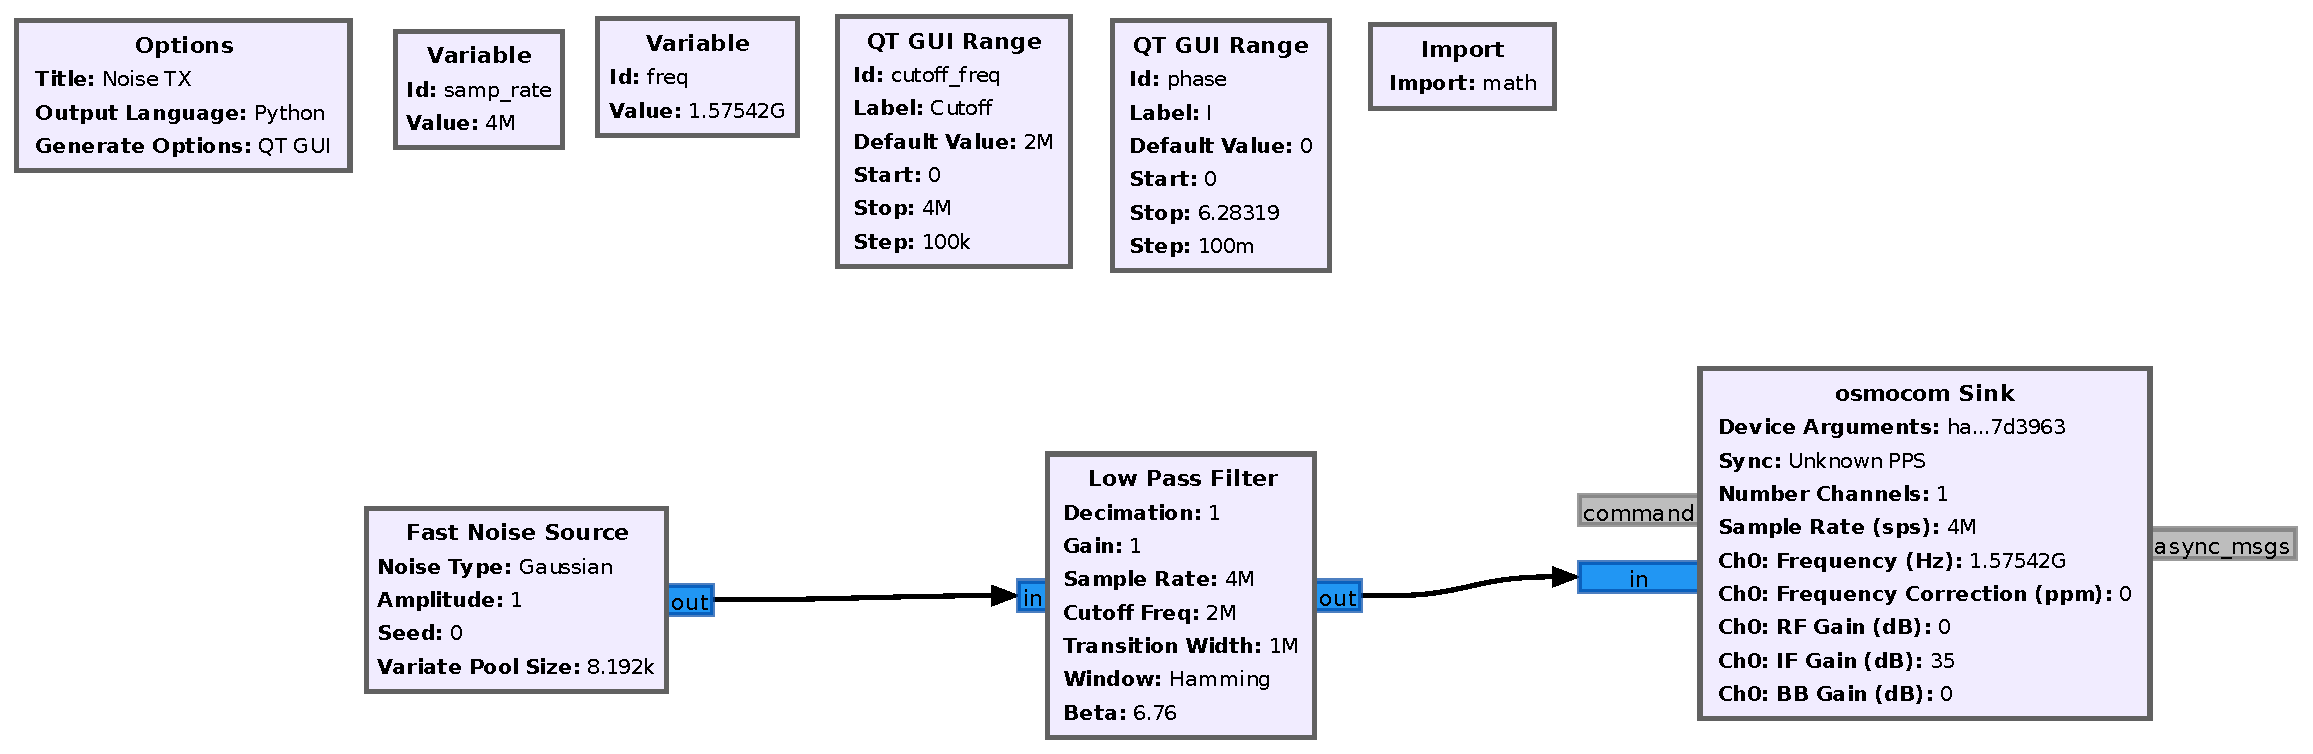
\includegraphics[angle=90, scale=0.5]{hackrf_tx_noise}
\par\end{centering}

\section{GNU Radio siųstuvo programa, pastoviam signalui generuoti}

\begin{centering}
    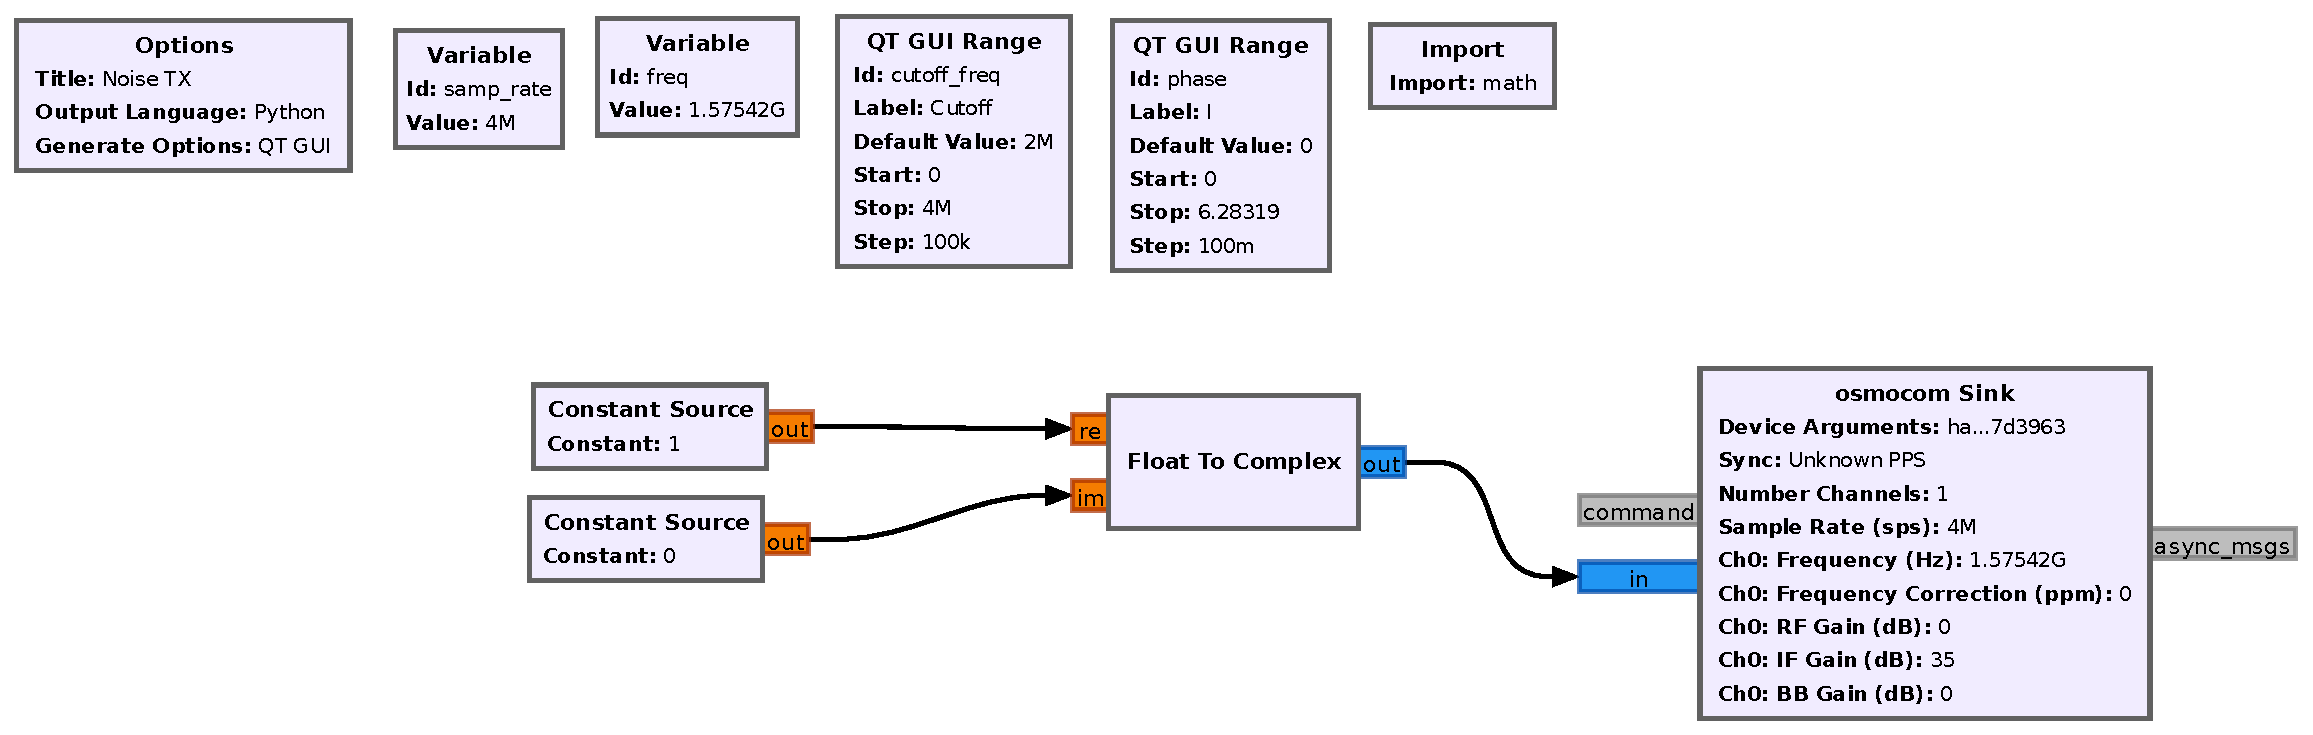
\includegraphics[angle=90, scale=0.5]{hackrf_tx}
\par\end{centering}

\section{GNU Radio programa, koreliacijos skaičiavimui}

\begin{centering}
    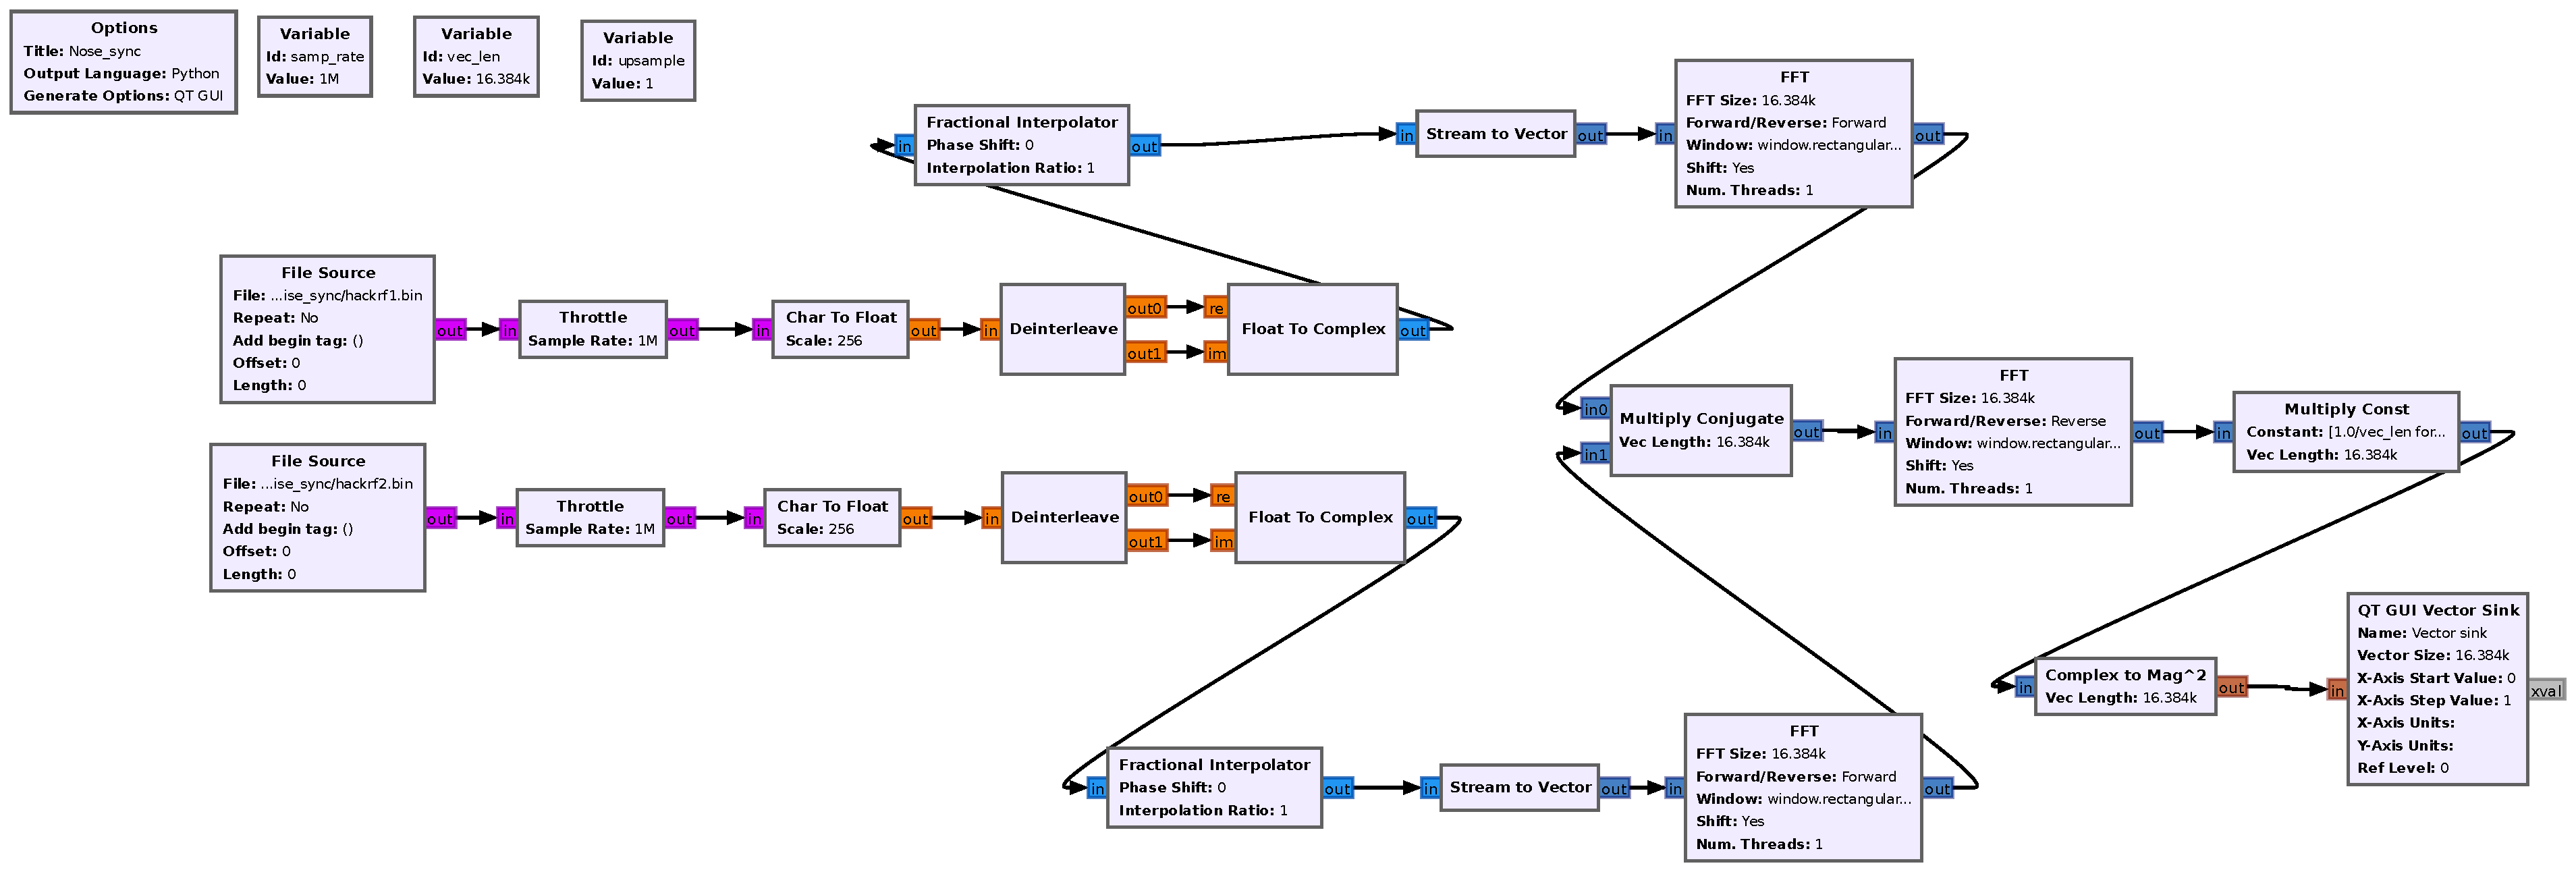
\includegraphics[angle=90, scale=0.32]{hackr_correlation}
\par\end{centering}


\end{document}
